% ==============================================================================
% TCC - Nome do Aluno
% Capítulo 3 - Avaliação do Trabalho
% ==============================================================================
\chapter{Experimentos e Resultados}
\label{cap-experimentos}

O \textit{p}Nota é um sistema que foi produzido com o andamento de experimentos em plataformas AVA na Universidade Federal do Espírito Santo (UFES). Nesse período, durante o desenvolvimento foram adicionadas diferentes técnicas para validar a capacidade de compreensão linguística e avaliativa do modelo SAG proposto. Os testes envolveram um conjunto de atividades com mais de 126 questões e 2805 respostas. Nestes testes foram analisadas formas distintas de escrita e em diferentes níveis de instrução, do Ensino Básico à Pós-Graduação, abordando tópicos distintos como Computação, Ciências, Filosofia, Economia e Medicina. Entretanto, para avaliar o sistema apresentamos aqui uma série de experimentos com \textit{datasets} encontrados na literatura.

Esse capítulo apresenta três séries de experimentos. A primeira avalia a parte fundamental da técnica de \textit{Active Learning} do sistema \textit{p}Nota, com o uso da \textit{clusterização} para a identificação dos principais itens de resposta em cada base de dados. A segunda apresenta os métodos de classificação, a qualidade do aprendizado do sistema na predição de notas e sua adequação ao modelo esperado pelo tutor. Por fim, o terceiro módulo reflete como os modelos de resposta são formados pelo sistema e apresentados como feedback aos alunos e professores.

\section{Base de Dados}
 Nove bases de dados foram selecionadas de acordo com a literatura, em português e inglês. Cada base de dados foi utilizada conforme as suas características. As bases de dados foram organizadas segundo o formato da nota, entre ordinais, discretas e contínua \cite{morettin2010}.

Em bases de dados com notas \textit{ordinais} o método avaliativo do tutor é dado de forma textual e categórica. A representação do rótulo não estabelece escalas para o sistema, não sendo possível mensurar a diferenças na escala \textit{a priori}. O modelo formado deve compreender as estruturas textuais de forma simbólica, caracterizando a essência de cada nível. Portanto, o classificador deve ser robusto para aprender a relevância das respostas pela equivalência de palavras-chave. Basicamente, é fundamental para o classificador produzir um modelo com as informações essenciais para a resposta receber tal categoria e reproduzir o modelo.

Por outro lado, outra situação acontece com bases de dados avaliados com notas contínuas. As notas \textit{contínuas} não apresentam níveis, mas sim intervalos numéricos. As respostas recebem notas de acordo com o intervalo avaliativo. Apesar de numérico, o fato da variável não definir uma categoria que represente a divergência entre respostas dificulta o aprendizado do modelo avaliativo. Ao sistema, isso torna subjetiva a espectativa de resposta subjetivo. Assim, esse tipo de atividade é avaliada por interpolação. Nesse caso, o sistema realiza uma regressão de acordo com os pontos conhecidos, gerando a nota pela referência ao grau de similaridade para as demais respostas.

Por fim, a avaliação \textit{discreta} numérica é a mais comum. Esse modelo favorece também os sistemas computacionais na criação da representação de resposta por categoria de nota. Ao tempo que a categoria induz a equivalência de todas as respostas ao qual foi associada. Assim, o sistema consegue mensurar equivalência e divergências pelos indícios de proximidade entre respostas avaliadas já conhecidas para além da mesma categoria. O desafio do sistema com este tipo de nota é criar um bom modelo de classificação que aprenda essa relação dupla. Para além da categoria das respostas, o sistema passa a ter que interpretar as informações fundamentais de cada classe e a escala de divergência para as demais categorias. A Tabela \ref{tab-datasets} apresenta os detalhes de cada \textit{dataset}, incluindo o número de questões, o total de respostas, o modelo avaliativo aplicado e a linguagem.

\begin{center}
\begin{table}[!h]
\begin{tabular}{r |c c c c} 
 \hline
 Base de Dados & Quest{\~o}es & Respostas & Modelo Avaliativo & Linguagem \\ \hline
 SEMEVAL2013 Beetle & 47 & 4380 & ordinal & Ingl{\^e}s \\
 SEMEVAL2013 SciEntsBank & 143 & 5509 & ordinal & Ingl{\^e}s \\
 Kaggle ASAP-SAS & 10 & 17043 & discreto & Ingl{\^e}s \\
 Powergrading & 10 & 6980 & discreto & Ingl{\^e}s \\
 UK Open University & 20 & 23790 & discreto & Ingl{\^e}s \\
 University of North Texas & 87 & 2610 & cont{\'i}nuo & Ingl{\^e}s \\
 Kaggle PTASAG & 15 & 7473 & discreto & Portugu{\^e}s \\
 Projeto Feira Liter{\'a}ria & 10 & 700 & discreto & Portugu{\^e}s \\
 VestUFES & 5 & 460 & cont{\'i}nuo & Portugu{\^e}s \\
 \hline
 \hline
\end{tabular}
\caption{Bases de dados e suas principais caracter{\'i}sticas.}
\label{tab-datasets}
\end{table}
\end{center}

A Tabela \ref{tab-datasets} descreve os nove \textit{datasets} utilizados nos experimentos deste capítulo. Através das características apresentadas, sabendo que cada \textit{dataset} contém uma quantidade regular de respotas, observamos a grande diversidade de quantidade de respostas por questão. Com questões de 30 até mais de 1800 respostas. É importante destacar ainda que, a definição de respostas curtas e as características textuais das respostas de cada um destes \textit{datasets} foram apresentadas no Capítulo \label{cap1-intro}, em especial na Tabela \ref{tab-features}. No total, esse \textit{corpora} apresenta um total de 337 questões e 61.268 respostas. Cada base de dados e sua descrição completa é apresentada a seguir:


\subsection{Base de Dados \textit{Beetle} do \textit{SEMEVAL'2013 : Task 7} \textit{(Inglês)}}
\label{beetle-db}

\textit{Beetle} \cite{dzikovska2012} é um dos \textit{datasets} utilizados durante o \textit{International Workshop on Semantic Evaluation - SEMEVAL'2013}. O \textit{SEMEVAL} seleciona anualmente uma série de desafios em análise semântica e apresenta no formato de competição. O \textit{corpus Beetle} foi selecionado para a \textit{Task 7: The Joint Student Response Analysis and 8th Recognizing Textual Entailment Challenge} \cite{dzikovska2013}. Portanto, a competição consistia em duas propostas. A primeira é a análise e avaliação das respostas obtidas e a segunda o reconhecimento da relação textual entre as respostas coletadas e a expectativa de resposta do professor.

Esse \textit{dataset} consiste em uma coleção de interações entre estudantes e o sistema \textit{Beetle II}. Beetle II é um Sistema Tutor Inteligente (STI) para aprendizado de conhecimentos básicos em Eletricidade e Eletrônica do Ensino Médio. Os alunos foram acompanhados durante 3 a 5 horas para preparar materiais, construir e observar circuitos no simulador e interagir com o STI. Esse sistema faz questões aos alunos, avalia as respostas e envia \textit{feedbacks} via \textit{chat}. Na construção deste \textit{dataset} foram acompanhados 73 estudantes voluntários da \textit{Southeastern University} dos Estados Unidos.

Foram aplicadas questões categorizadas em dois tipos factuais e explicativas. As questões factuais requerem que o aluno nomeie diretamente determinados objetos ou propriedades. Equanto isso, as questões explicativas demandam que o aluno desenvolva a resposta em uma ou duas frases. Para a formação do \textit{dataset} foram adicionadas apenas as atividades do segundo tipo, pois representam maior complexidade para sistemas computacionais. No total foram selecionadas 47 questões com 4380 respostas. A avaliação foi feita conforme o domínio demonstrado sobre o assunto em cinco categorias: \textit{correct}, \textit{partially-correct-incomplete}, \textit{contradictory}, \textit{irrelevant} e \textit{non-domain}. Durante a anotação o coeficiente \textit{Kappa} obtido foi de 69\% de concordância.


\subsection{Base de Dados \textit{SciEntsBank} do \textit{SEMEVAL'2013 : Task 7} \textit{(Inglês)}}
\label{scientsbank-db}

O \textit{corpus Science Entailments Bank (SciEntsBank)} \cite{dzikovska2012} é um dos \textit{datasets} utilizados durante o \textit{International Workshop on Semantic Evaluation - SEMEVAL'2013} \cite{dzikovska2013}, com foco na avaliação de sistemas conforme a sua capacidade de análise e exploração semântica da linguagem. É uma base de dados formadas pela avaliação de questões da disciplina de Ciências. Na avaliação 16 assuntos distintos são abordados entre ciências físicas, ciências da terra, ciências da vida, ciências do espaço, pensamento científico e tecnologia. 

As questões são parte da \textit{Berkeley Lawrence Hall of Science Assessing Science Knowledge (ASK)} com avaliações padronizadas de acordo com o material de apoio \textit{Full Option Science System (FOSS)}. Participaram estudantes dos Estados Unidos de terceira a sexta série, coletando em torno de 16 mil respostas. Porém, dentre as questões de preenchimento, objetivas e discursivas, foram utilizadas apenas as discursivas, que requisitavam explicações dos alunos segundo o tema. As respostas foram graaduadas em cinco notas ordinais: \textit{correct}, \textit{partially-correct-incomplete}, \textit{contradictory}, \textit{irrelevant} e \textit{non-domain}. Portanto, o \textit{SciEntsBank} consiste em um conjunto com 143 questões selecionadas e 5509 respostas. No processo de avaliação foi observado o coeficiente \textit{Kappa} com 72.8\% de concordância.

\begin{comment}
[('contradictory', 557), ('correct', 2241), ('irrelevant', 1248), ('non_domain', 26), ('partially_correct_incomplete', 1437)] 5509 SCIENTSBANK

[('contradictory', 1160), ('correct', 1841), ('irrelevant', 130), ('non_domain', 218), ('partially_correct_incomplete', 1031)] 4380 BEETLE 
\end{comment}

\subsection{Base de Dados do Concurso ASAP-SAS no \textit{Kaggle} \textit{(Inglês)}}
\label{kaggle-db}

A base de dados \textit{ASAP - SAS}, \textit{Automated Student Assessment Prize - Short Answer Scoring} é uma competição proposta pela \textit{Hewllet Foundation} na plataforma \textit{Kaggle} \footnote{The Hewlett Foundation - Short Answer Scoring: https://www.kaggle.com/c/asap-sas}. A \textit{ASAP} consistiu em três fases:

\begin{itemize}
\item Fase 1:  Demonstração em respostas longas (redações); 
\item Fase 2:  Demonstração em respostas curtas (discursivas);
\item Fase 3:  Demonstração simbólica matemática/lógica (gráficos e diagramas).
\end{itemize}

O objetivo da competição foi descobrir novos sistemas de apoio ao desenvolvimento de escolas e professores. Especificamente, as três fases destacam a atividade lenta e de alto custo de avaliar manualmente testes, mesmo que com padrões bem definidos. Uma consequência disso é a redução do uso de questões discursivas nas escolas, dando preferência para as questões objetivas para evitar a sobrecarga de trabalho. Isso evidencia uma gradativa redução da capacidade dos professores em incentivar o pensamento crítico e as habilidades de escrita. Portanto, os sistemas de apoio, são uma possível solução para suportar os métodos de correção, avaliação e feedback ao conteúdo textual dos alunos.

Neste contexto, a competição apresentou 10 questões multidiciplinares, de ciências à artes. Estão distribuidas 17043 respostas de alunos dentre essas atividades. Para chegar nessa quantidade, foram selecionadas por volta de 1700 respostas dentre 3000 respostas em cada atividade. Cada resposta tem aproximadamente 50 palavras. A primeira avaliação foi dada pelo primeiro especialista como nota final e a segunda nota foi atribuída apenas para demonstrar o nível de confiança da primeira nota. A avaliação apresentada por dois especialistas apresentou concordância de 90\% no coeficiente \textit{Kappa}.


\subsection{Base de Dados \textit{Powergrading} \textit{(Inglês)}}
\label{powergrading-db}
Elaborado através do \textit{United States Citizenship Exam} (USCIS) em 2012, a base de dados \textit{Powergrading} contém 10 questões e 6980 respostas \cite{basu2013}. Desenvolvida originalmente para destacar a possibilidade de avaliação massiva, o \textit{dataset} selecionou 698 respostas para cada uma das questões. As respostas foram geradas com \textit{Amazon Mechanical Turk}, serviço remoto de análise manual de conteúdo para anotação da \textit{Amazon}. Foi coletada por um grupo de pesquisa da \textit{Microsoft}\footnote{Powergrading: https://www.microsoft.com/en-us/download/details.aspx?id=52397} e cada questão acompanha um modelo de resposta e as respostas recebidas para cada questão.  Além disso, acompanha o \textit{dataset} outras 10 questões não avaliadas.

Foram requisitadas respostas com poucas palavras, atingindo no máximo uma ou duas sentenças. Por conta disso, os resultados são respostas muito curtas com 4 palavras em média. Em geral, por conta da convergência, vários padrões de resposta se repetem \cite{riordan2017}. Com avaliações binárias, 1 para resposta correta e 0 para incorreta, cada resposta apresenta avaliações de três diferentes tutores. Apesar de alguns trabalhos assumirem um dos avaliadores como padrão, utilizamos como modelo de avaliação a resultante da comparação entre os três. Apesar de não ter complexidade linguística, ocorreu contradição entre os avaliadores em 470 respostas. Em valores percentuais, isso representa 7\% do total de respostas do conjunto de dados.

\begin{comment}
Respostas não coincidentes em cada questão
q1 - 1 q2 - 12 q3 - 145 q4 - 45 q5 - 18 q6 - 52 q7 - 20 q8 - 17 q13 - 108 q20 - 52
\end{comment}

\subsection{Base de Dados da \textit{UK Open University} \textit{(Inglês)}}
\label{openunv-db}

A base de dados da \textit{UK Open University} é um conjunto de questões coletadas na disciplina de introdução à ciências, denominada \textit{S103 - Discovering Science} \cite{jordan2012}. O foco do conjunto de atividades são abordagens em questões factuais bem concisas, não excedendo 20 palavras. Os alunos receberam as atividades através do ambiente da \textit{Intelligent Assessment Technologies (IAT)}, o \textit{FreeText Author}. O \textit{FreeText Author} foi utilizado como um método de \textit{CAA} de modo interativo e com resultado automático analizando a resposta do aluno segundo os padrões de resposta conhecidos. O sistema permitiu uma sequência de envios e apresentava comentários da resposta como \textit{feedback} para os alunos. Dependendo da complexidade da resposta, o tempo de retorno dos resultado varia muito entre alguns poucos minutos até mais do que um dia.

Dentre as 20 questões, esse \textit{dataset} apresenta diferentes quantidades de respostas entre 511 e 1897. A avaliação é discreta e binária, definindo cada resposta como correta ou incorreta. Não existe notas intermediárias, representando diretamente se o aluno atendeu ou não os requisitos da resposta.


\subsection{Base de dados da \textit{University of North Texas} \textit{(Inglês)}}
\label{ntexasunv-db}

O \textit{dataset} da \textit{University of North Texas - UNT} \cite{mohler2011}, conhecido como \textit{Texas dataset} \footnote{Texas Dataset: https://web.eecs.umich.edu/{\textasciitilde}mihalcea/downloads.html}, é uma coleção de questões discursivas extraída no curso de Ciência da Computação. Composta por 80 atividades únicas, esse conjunto é composto por dez listas de exercícios com até sete questões e dois testes com dez questões cada. Foram aplicados em um ambiente virtual de aprendizagem durante a disciplina de Estrutura de Dados para 31 alunos. No total o \textit{dataset} é composto por 2273 respostas de alunos dentre as 80 atividades.

A avaliação foi feita com cinco notas discretas, de 5 equivalente a resposta perfeita até 0 completamente incorreta. Foram avaliadas por dois avaliadores independentes, estudantes do curso de Ciência da Computação. Para os autores, o modelo seguido pelo sistema deve ser a resultante da média ente os avaliadores, em intervalo contínuo. Dentre as notas atribuídas, 57,7\% das respostas receberam a mesma nota. Enquanto isso, um nível de diferença entre as notas representou 22,9\% do total de respostas. Foi constatado também que, dentre as diferenças na avaliação, o avaliador 1 atribuia maiores notas 76\% das vezes.

\subsection{Base de dados \textit{PTASAG} no \textit{Kaggle} \textit{(Português)}}
\label{ptasag-db}

A \textit{PTASAG - Portuguese Automatic Short Answer Grading Data} é uma base de dados brasileira apresentada por \cite{galhardi2018b} e disponibilizada na plataforma \textit{Kaggle} \footnote{PT-ASAG-2018: https://www.kaggle.com/lucasbgalhardi/pt-asag-2018}. Foi coletada pela Universidade Federal do Pampa - Unipampa em conjunto com cinco professores de biologia do Ensino Fundamental. Foram criadas 15 atividades com base no sistema Auto-Avaliador CIR. Em biologia, os tópicos abordados foram sobre o corpo humano. Cada questão acompanha uma lista de conceitos, as respostas avaliadas e as respostas candidatas criadas pelos professores como referência. Foram criadas entre duas e quatro respostas candidatas contendo entre três e seis palavras-chave.

As atividades foram aplicadas ao Ensino Fundamental para 326 estudantes de 12 a 14 anos do 8\textsuperscript{\b{o}} e 9\textsuperscript{\b{o}} ano. Somados a estes, também foram aplicados a 333 alunos do Ensino Médio de 14 a 17 anos. As respostas foram avalidas por 14 estudantes de uma turma do último ano, considerando uma escala de notas de 0 a 3:

\begin{itemize}
\item Nota 0: Majoritariamente incorreta, fora de tópico ou sem sentido;
\item Nota 1: Incorreta ou incompleta mas com trechos corretos;
\item Nota 2: Correta mas com importantes trechos faltantes;
\item Nota 3: Majoritariamente correta apresentando os principais pontos.
\end{itemize}

No total, participaram 659 estudantes com um total de 7473 respostas. Cada uma das 15 questões apresenta entre 348 e 615 respostas. Apenas 4 questões foram avalidas por mais de um avaliador para verificar a concordância entre avaliadores. O coefficiente \textit{Kappa} observado foi de, em média, 53.25\%.


\subsection{Base de Dados do Projeto Feira Literária das Ciências Exatas \textit{(Português)}}
\label{findes-db}

É um conjunto de dados coletados durante o Projeto Feira Literária das Ciências Exatas \cite{nascimento2020}. As questões foram obtidas durante uma Atividade Experimental Problematizada por meio de um livro paradidático, ou seja, cujo objetivo primário não é o apoio didático. O livro escolhido foi \textit{A Formula Secreta} de David Shephard. 

Conforme o livro, os professores formularam 10 atividades e ministraram para 70 alunos do 5º ano de Ensino Fundamental. Essas atividades ministradas descreviam situações práticas de Química básica. No total, o conjunto de dados conta com 10 questões, 700 respostas e suas respectivas avaliações.


\subsection{Base de Dados do Vestibular UFES \textit{(Português)}}
\label{vest-ufes-db}

A base de dados VestUFES \cite{pissinati2014} é uma amostra das questões discursivas de Português do vestibular da UFES em 2012. A amostra selecionada contém 460 respostas divididas igualmente entre as 5 questões de língua portuguesa, também referentes a respostas dadas por 92 diferentes alunos.

Cada resposta foi avaliada por dois avaliadores. De acordo com o vestibular da universidade, os a avaliadores atribuíram notas entre 0 e 2 pontos em cada questão, totalizando 10 na soma da prova. Caso houvesse divergências de mais de 1 ponto entre as correções um terceiro avaliador era acionado para reavaliar a coerência das notas. A nota das respostas do \textit{dataset} foram redimensionadas pelo autor para o intervalo de 0 a 10 pontos. Na nova escala, as diferenças observadas entre os avaliadores foi de, em média, 1,38 pontos com desvio padrão de 1,75.


\begin{comment}
\subsection{Base de Dados das Disciplinas UFES \textit{(Português)} \label{disciplinas-ufes-db}
Essa base de dados foi coletada de algumas disciplinas ministradas na Universidade Federal do Espírito Santo - UFES entre 2015 e 2016 através do Moodle do Laboratório Computação de Alto Desempenho - LCAD. Entre as disciplinas estão Metodologia e Técnicas de Pesquisa Científica, Filosofia e Tecnologia da Informação II. Totalizando 45 atividades, neste \textit{dataset} foram recebidas 1162 submissões com média 25,82 e desvio padrão de 13,54 respostas por atividade.

O diferencial dessa base de dados é a mudança de características nas respostas encontradas nas múltiplas disciplinas, professores e alunos. Observam-se alterações consideráveis quanto ao tamanho, número de grupos, critério avaliativo ou objetividade. 
\end{comment}


\section{Experimentos}
\label{sec-experimentos}

A série de experimentos realizados têm como intúito demonstrar o uso do \textit{p}Nota, em conjunto com o professor, de forma a criar modelos com bom desempenho na atribução de notas. Além disso, através dos \textit{datasets} conhecidos na literatura, podemos comparar a proposta de análise de estruturas textuais com os principais trabalhos publicados. Em uma primeira comparação avaliaremos a qualidade dos \textit{clusters} formados. Na sequência, apresentamos comparativos com as técnicas utilizadas na literatura nos desafios de uma forma geral. E, por fim, verificamos o desempenho do sistema quanto ao ganho de informação, em uma forma de validar a capacidade de aprendizado do modelo linguístico.

\subsection{Resultados de \textit{Clusterização}}
\label{sec-res-clustering}

Em uma primeira análise, observamos o processo de \textit{clusterização} através do propósito da aplicação em \textit{Active Learning}. 



os resultados dos \textit{clusters} formados para os conjuntos de atividades através do processo de otimização \cite{spalenza2019}. Os resultados obtidos, visando ter \textit{clusters} mais homogêneos após a otimização, são caracterizados pela 



Analisamos os resultados segundo três métricas de informação e o grau de similaridade entre grupos. Para isso, utilizamos as métricas ARI, NMI e CA, descritas na Seção \ref{subsec-clusterizacao}. Os resultados médios obtidos para os conjuntos de dados são apresentados na Tabela \ref{tab-clstr-index}.

\begin{table}[!h]
\begin{center}
\begin{tabular}{r | r r r }
 \hline

\textit{Dataset}  & CA & HS & CS \\ \hline 
SEMEVAL2013 Beetle & 0,5521 & 0,1127 & 0,3128 \\
SEMEVAL2013 SciEntsBank SciEntsBank & 0,5747 & 0,1152 & 0,2071 \\
UK Open University  & 0,7604 & 0,1752 & 0,0647 \\
Projeto Feira Liter{\'a}ria & 0,5529 & 0,0848 & 0,2896 \\
Kaggle ASAP-SAS   & 0,5215 & 0,0216 & 0,0801 \\
Powergrading & 0,8537 & 0,3747 & 0,1331 \\
Kaggle PTASAG  & 0,4863 & 0,0732 & 0,1663 \\
University of North Texas & - & - & - \\
VestUFES & - & - & - \\
 \hline
\end{tabular}
\end{center}
\caption{Bases de dados e índices qualitativos de \textit{clusterização}.}
\label{tab-clstr-index}
\end{table}

A Tabela \ref{tab-clstr-index} demonstra que, apesar da baixa relação entre \textit{clusters} e sua representação direta como rótulos, temos excelentes resultados quanto à classificação. Isso indica que o sistema apresenta uma capacidade de particionamento dos dados em núcleos distintos de uma mesma classe. Na prática, uma categoria é representada por mais que um \textit{cluster}, seja formado por \textit{outliers} (até 10 amostras), grupos com pares de categorias ou grupos com padrões consistentes. Um quarto tipo seriam os grupos com padrões aleatórios agrupados, em geral não desejável. Neste último caso, os resultados não contribuem muito para a passagem de informações entre as etapas de amostragem por \textit{clusterização} e classificação. Com alinhamento direto ao método de \textit{clusterização} proposto pelos autores, o \textit{dataset Powergrading} apresentou alto desempenho logo de partida com nosso método. Por outro lado, com grande gradação de notas, os \textit{datasets} do \textit{SEMEVAL Beetle} e \textit{SciEntsBank} indicam grande complexidade quanto a homogeneidade dos grupos. Para destacar essa distinção entre os grupos e o conteúdo, apresentamos a diferença entre \textit{centróides} na Figura \ref{fig-hmPowergrading}.


\begin{figure}[!h]
\begin{minipage}[t]{.5\textwidth}
\centering
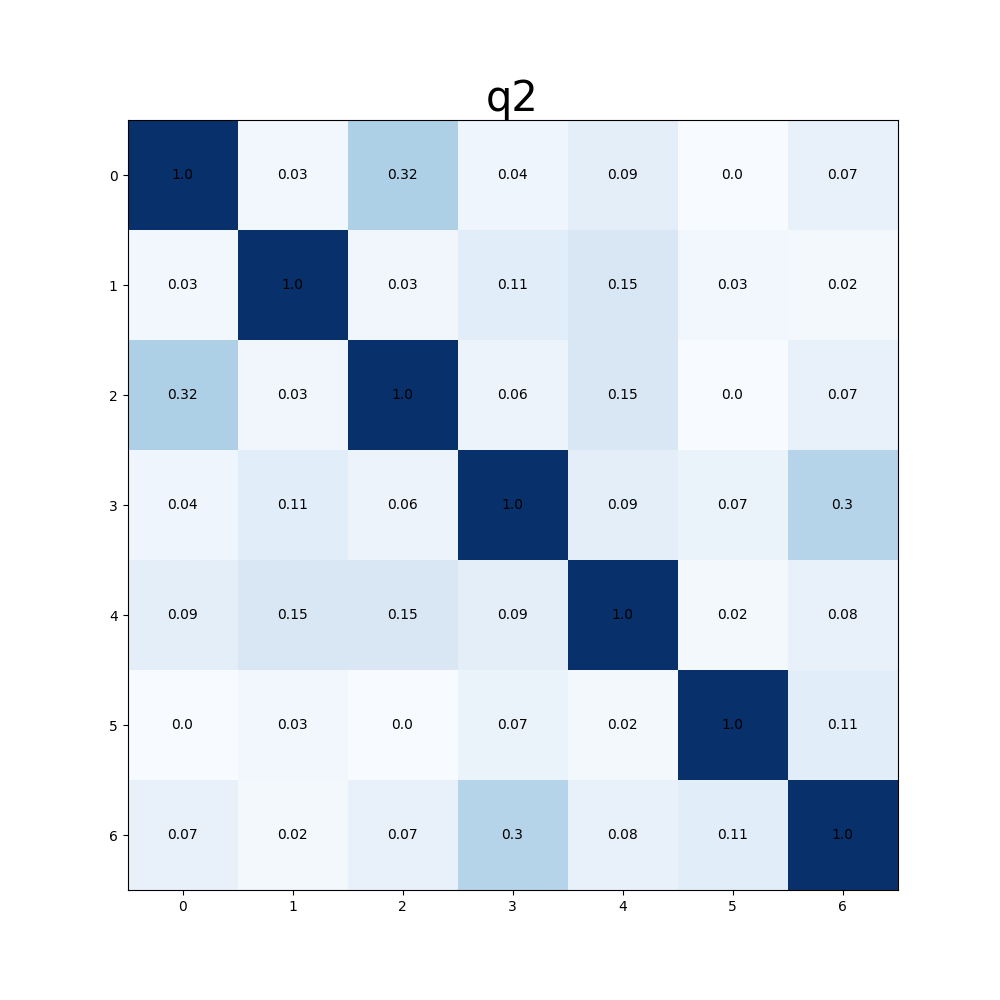
\includegraphics[width=\textwidth]{figuras/hmq2.png} 
\end{minipage}%
\begin{minipage}[t]{.5\textwidth}
\centering
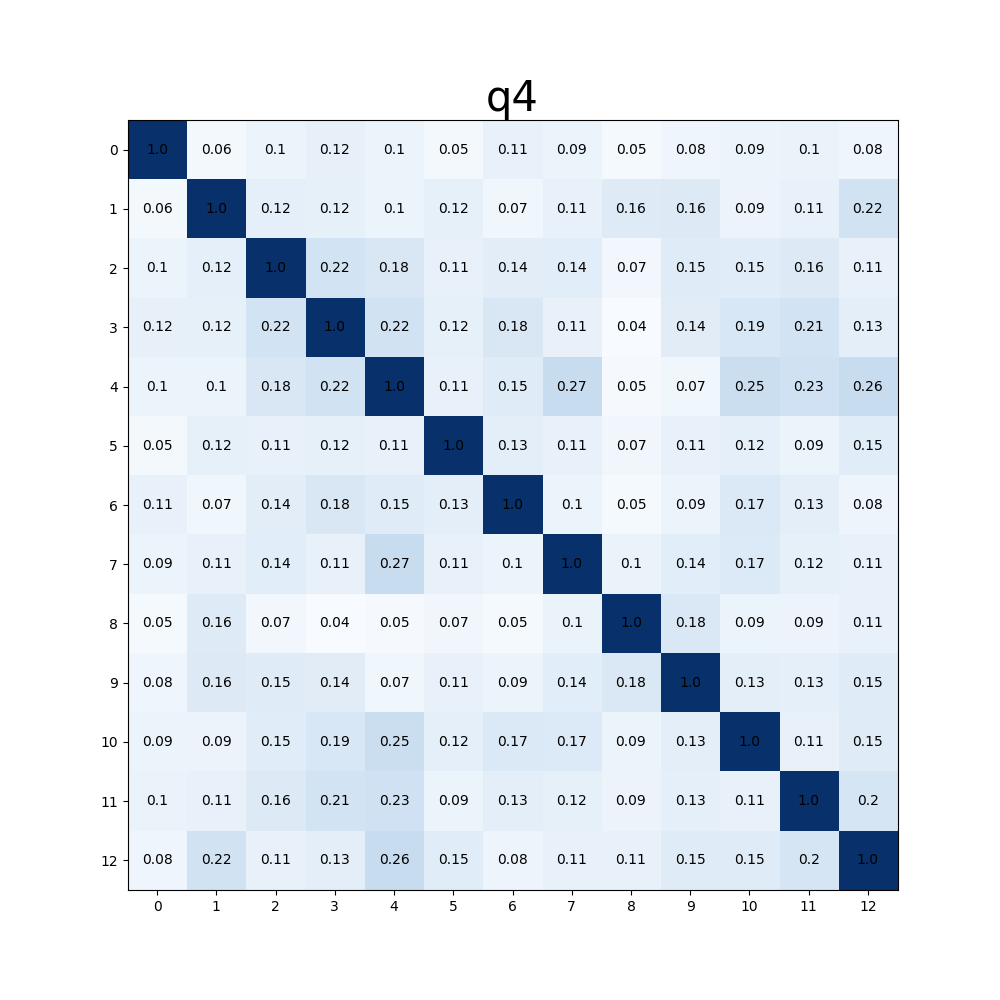
\includegraphics[width=\textwidth]{figuras/hmq4.png}
\end{minipage}%
\hfill
\begin{minipage}[t]{.5\textwidth}
\centering
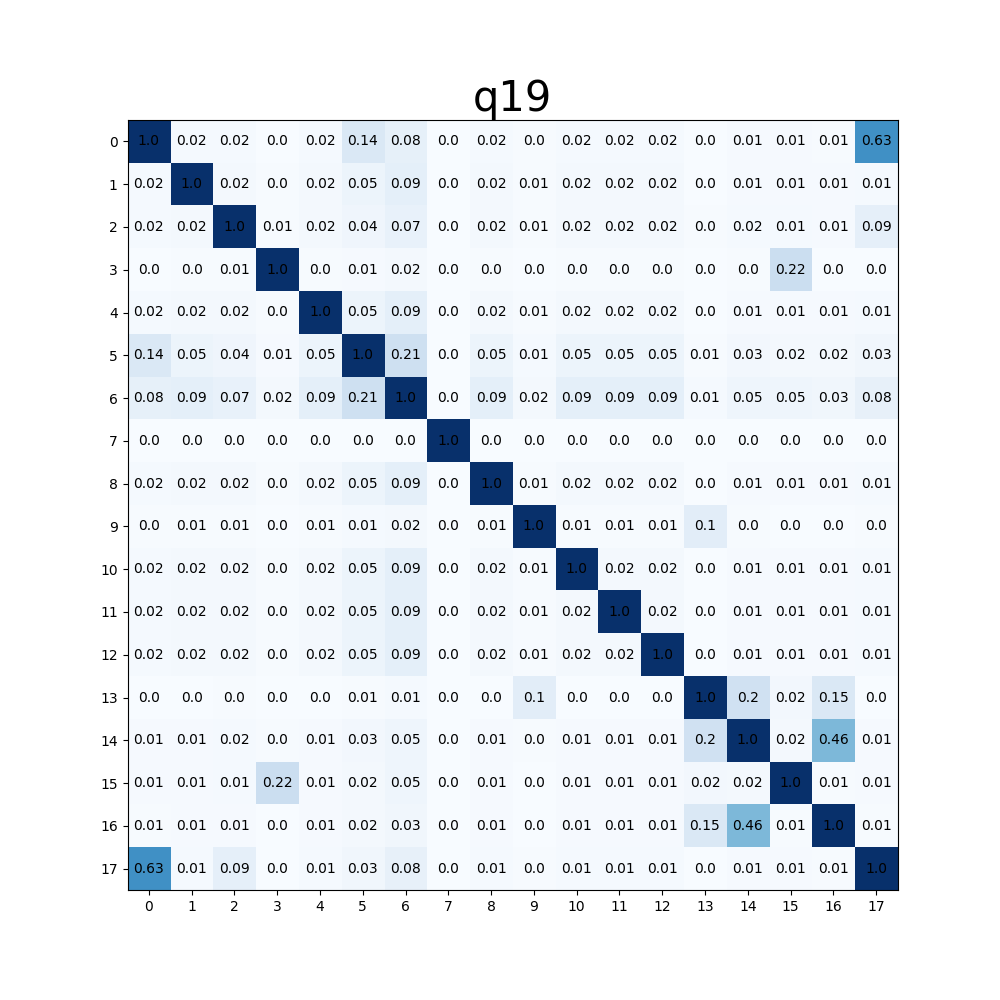
\includegraphics[width=\textwidth]{figuras/hmq19.png}
\end{minipage}%
\begin{minipage}[t]{.5\textwidth}
\centering
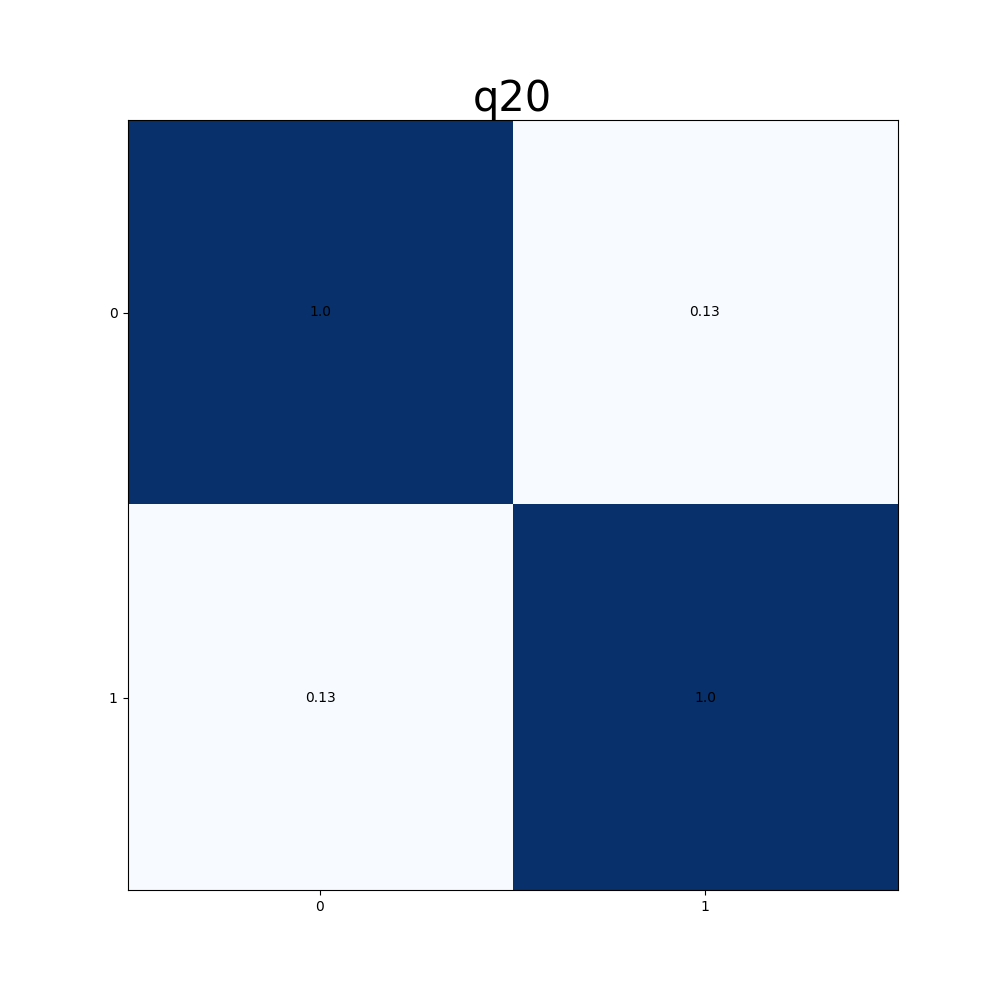
\includegraphics[width=\textwidth]{figuras/hmq20.png}
\end{minipage}
\caption{Similaridade entre \textit{centróides} para as atividades q2, q4 e q19 e q20 em \textit{Powergrading}.}
\label{fig-hmPowergrading}
\end{figure}

Como observamos nas imagens apresentadas na Figura \ref{fig-hmPowergrading}, existe a formação de grupos muito coesos. Essa coesão é explícita pela divergência do item médio (\textit{centróide}) os demais grupos. Como vemos através da matriz, em geral os índices de similaridade são menores que 0,25. Além disso, as atividades q2, q4, q19 e q20 apresentam respectivamente CA de 0,878, 0,805, 1,000 e 0,973. Isso demonstra a formação grupos divergentes mas com forte relação com a classe de nota. Para extração de padrões isso significa resultados de alta qualidade diretamente nos clusters formados. De certa forma este caso é incomum, ao qual esperamos lidar até com resultados de menor consistência nos \textit{clusters}. Denominamos agrupamentos consistentes aqueles que estão diretamente alinhados com a categoria atribuída. Entretanto, o cenário encontrado neste \textit{dataset} é o melhor possível, com padrões de resposta bem dispostos em \textit{clusters}. O caso oposto é dado pela diferença entre \textit{centróides} na Figura \ref{fig-hmSciEntsBank}.


\begin{figure}[!h]
\begin{minipage}[t]{.5\textwidth}
\centering
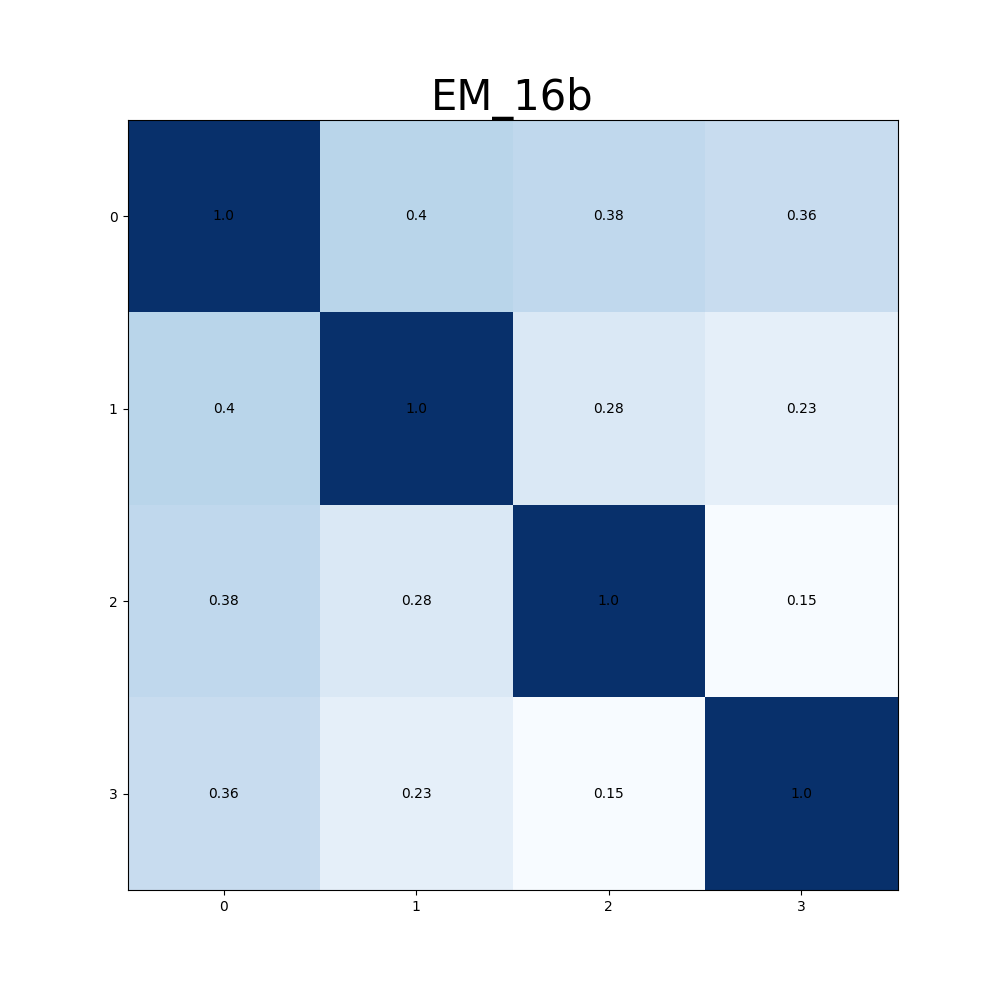
\includegraphics[width=\textwidth]{figuras/hmEM16b.png} 
\end{minipage}%
\begin{minipage}[t]{.5\textwidth}
\centering
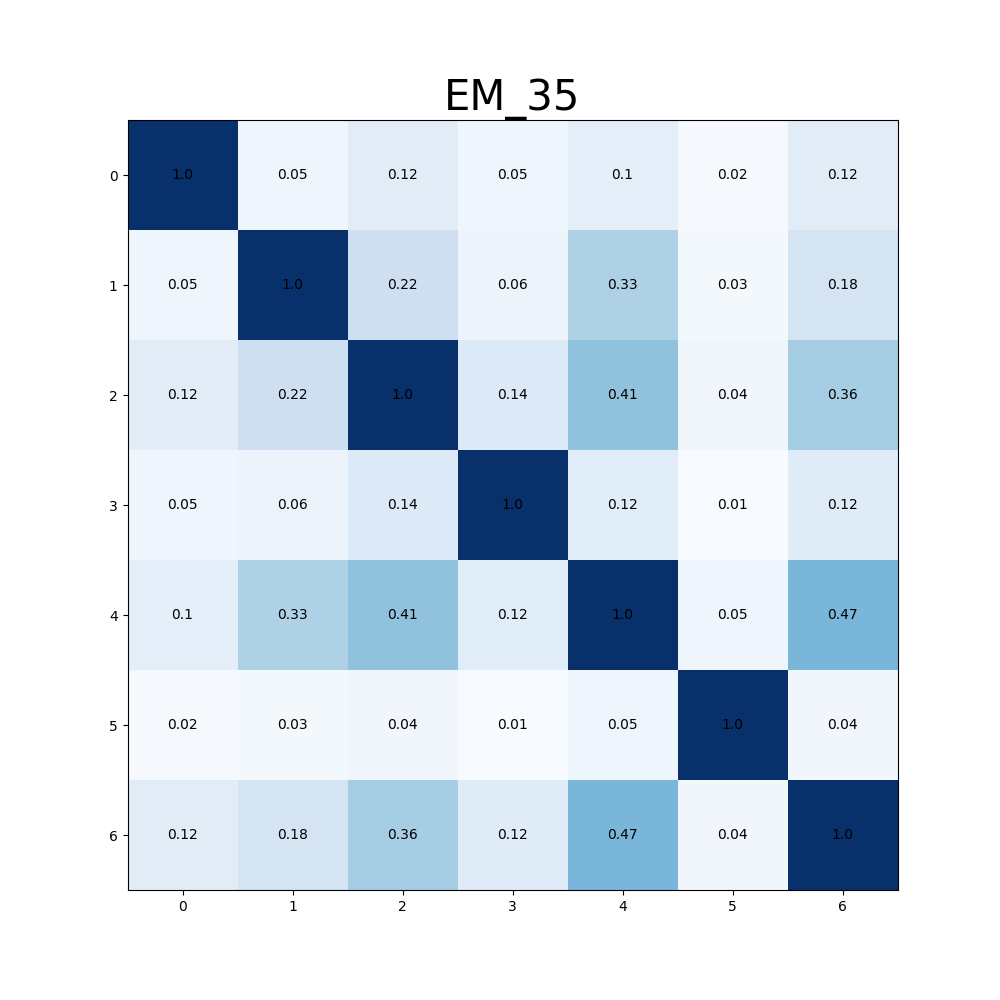
\includegraphics[width=\textwidth]{figuras/hmEM35.png}
\end{minipage}%
\hfill
\begin{minipage}[t]{.5\textwidth}
\centering
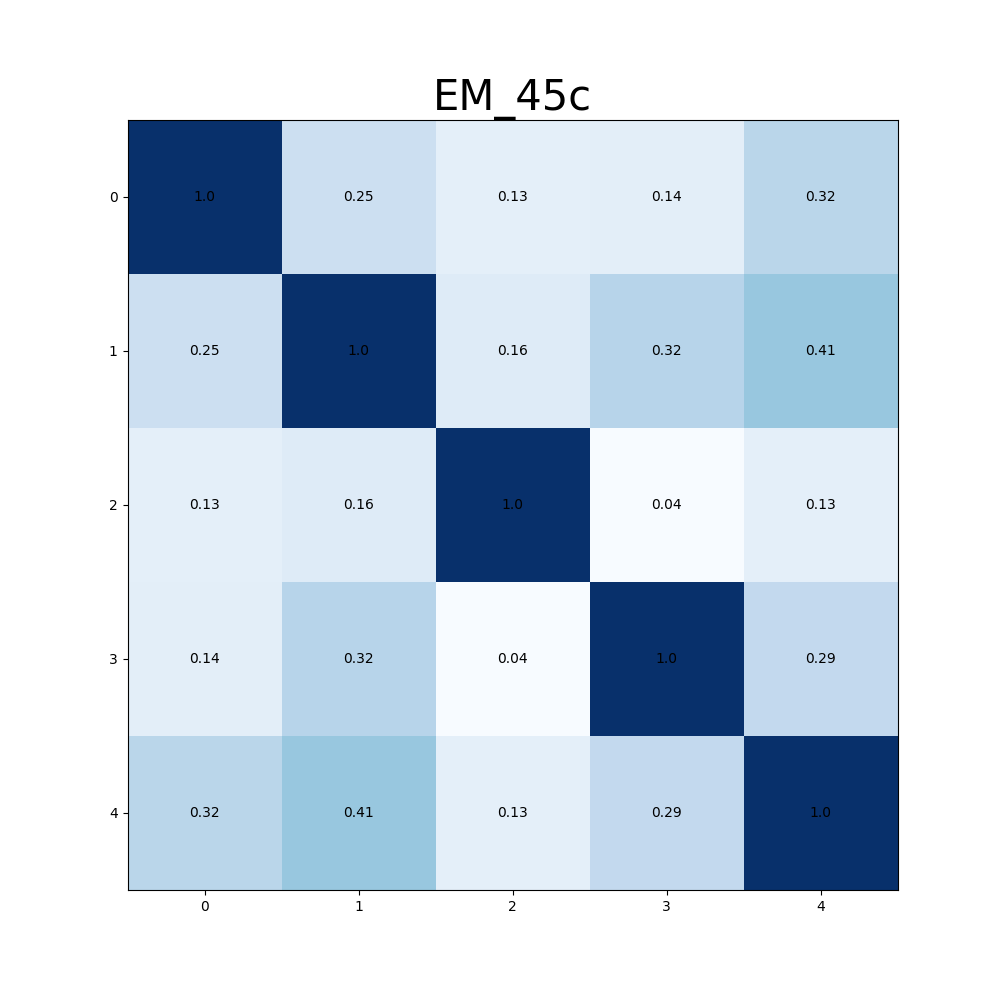
\includegraphics[width=\textwidth]{figuras/hmEM45c.png}
\end{minipage}%
\begin{minipage}[t]{.5\textwidth}
\centering
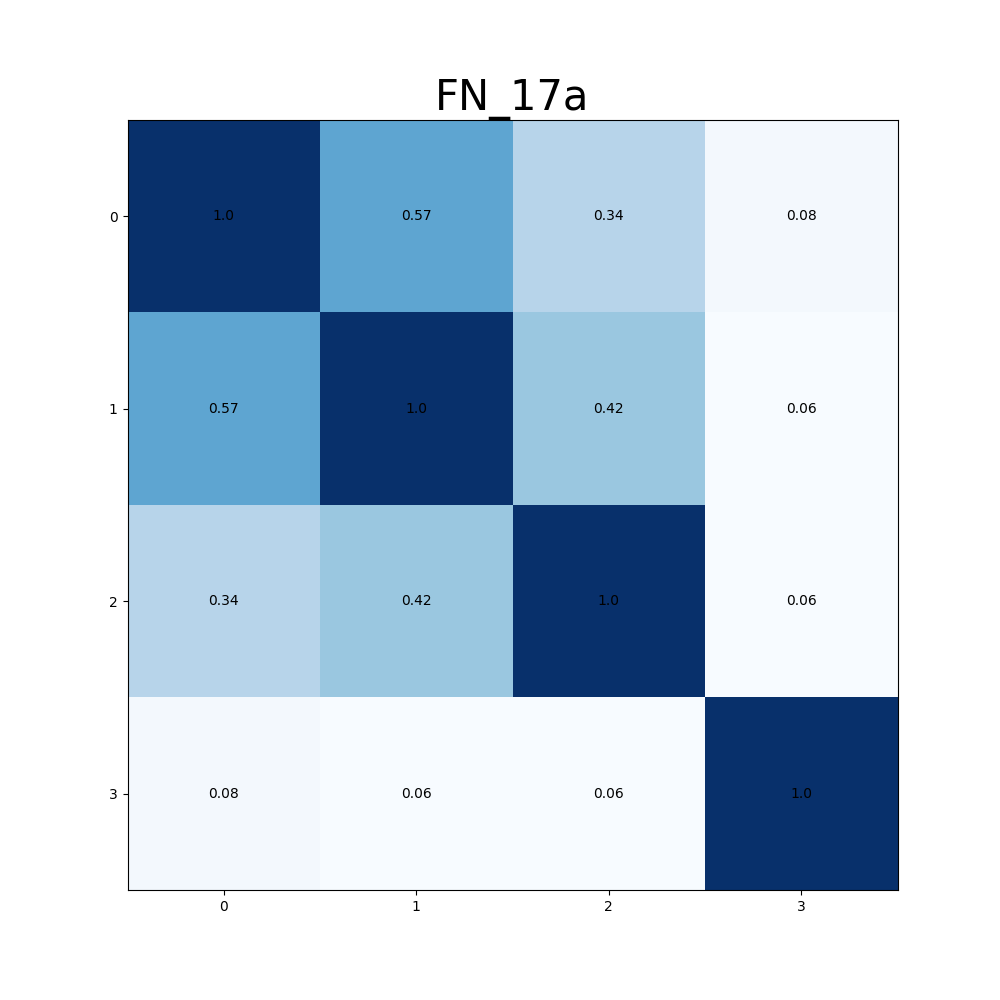
\includegraphics[width=\textwidth]{figuras/hmFN17a.png}
\end{minipage}
\caption{Similaridade entre \textit{centróides} para as atividades EM-16b, EM-35, EM-45c e FN-17a em \textit{SciEntsBank}.}
\label{fig-hmSciEntsBank}
\end{figure}

Como observamos na Figura \ref{fig-hmSciEntsBank}, as atividades EM-16b, EM-35, EM-45c e FN-17a apresentam regiões de maior similaridade. Diferentemente do que foi notado na atividade anterior, neste temos algumas áreas coincidentes, acima de 0,35 destacadas em azul. As áreas em azul indicam um grau grande de similaridade entre centróides dos grupos e, por consequência, são compatíveis em certo nível. Por conta disso, podemos considerar que tais grupos podem ter diferentes perspectivas de uma mesma classe ou mesclar diferentes classes. Por consequência, em ambos os casos, torna-se maior a responsabilidade do classificador \textit{a posteriori}, para designar padrões refinados para tais \textit{clusters}. Por outro lado, os resultados em CA para as atividades EM-16b, EM-35, EM-45c e FN-17a são de 0,425, 0,625, 0,825 e 0,700 respectivamente. Notamos que as quatro atividades representam diferentes níveis em CA, inclusive com avaliações não coincidentes. Alinhado a isso, é fundamental que o classificador seja responsável por refinar o reconhecimento de padrões estabelecido na \textit{clusterização}, elevando o nível dos resultados alcançados.

\subsection{Resultados de \textit{Classificação}}
\label{sec-res-classificacao}

Após resultados bem sucedidos na \textit{clusterização}, com CA por voto majoritário com médias superiores à 50\%, realizamos a análise dos resultados de classificação. Tais experimentos caracterizam-se pela simetria com a maioria das publicações e desafios lançados em avaliação de respostas discursivas \cite{burrows2015}. Nestes encontramos um particionamento de 75\% de respostas selecionadas para treinamento e validação dos modelos e 25\% para avaliação do desempenho das propostas. No caso deste trabalho, as partições iniciais dos \textit{datasets} foram desconsideradas por conta da seleção de amostras de modo semi-supervisionado. Portanto, neste trabalho a amostragem dos 75\% foi realizada conforme a distribuição dos itens nos \textit{clusters} formados, como relatado em detalhes na Seção \ref{sec-amostragem}. Portanto, foram mantidos tais percentuais como limiar superior dos sistemas. Vale ressaltar que esse processo ainda representa uma redução considerável do trabalho de correção nos mesmos 25\%, apesar da maioria dos dados ser designada para avaliação do professor.

Seguindo a característica da avaliação, vamos apresentar os resultados obtidos segundo a forma avaliativa adotada pelos professores. De forma mais complexa, temos os conjuntos de dados \textit{Beetle} e \textit{SciEntsBank} avaliados em 5 categorias textuais (ordinais) que indicam a completude da resposta conforme a expectativa do professor. Nesse aspecto, os \textit{datasets} do evento \textit{SEMEVAL' 2013}, apresentam 3 níveis de desafios. O primeiro nível é a avaliação de respostas não conhecidas, selecionadas aleatóriamente no conjunto de respostas (\textit{Unseen Answers}). O segundo nível compreende a correção de respostas em questões desconhecidas, ainda em um determinado domínio (\textit{Unseen Questions}). E, por fim, o terceiro nível está relacionado a análise de respostas em um domínio desconhecido (\textit{Unseen Domain}). Assim como a maioria dos sistemas SAG, o desafio que se enquadra no tópico aqui abordado é o primeiro (\textit{Unseen Answers}), avaliando conjuntos de respostas dentro de um mesmo tópico. 

Com destaque para o desbalanceamento dos dados \cite{dzikovska2013}, ambos os \textit{datasets} foram anotados em 5 categorias: \textit{correct}, \textit{partially-correct-incomplete}, \textit{contradictory}, \textit{irrelevant} e \textit{non-domain}. Evidenciamos ainda a complexidade, inclusive semântica, para separar as três categorias inferiores, \textit{contradictory}, \textit{irrelevant} e \textit{non-domain}. Utilizando os 6 classificadores descritos na Seção \ref{subsec-classificacao}, apresentamos os resultados obtidos na Tabela \ref{tab-SEMEVAL75}.

\begin{table}[!h]
\begin{center}
\begin{tabular}{l r r r r r r r}
    \hline
    \multicolumn{7}{l}{\textbf{Beetle}} &  (5 Categorias) \\ \hline
     & \multicolumn{7}{c}{M{\'e}tricas} \\

     & ACC & PRE & REC & F1(m) & F1(w) & Kappa(ln) & Kappa(qu) \\ \cline{2-8}
DTR & 56,26\% & 31,22\% & 31,27\% & 30,43\% & 55,32\% & 0,1026 & 0,0802 \\
GBC & 59,39\% & \textbf{36,56\%} & 35,08\% & 34,64\% & \textbf{59,28\%} & \textbf{0,1841} & \textbf{0,1990} \\
KNN & 55,79\% & 32,95\% & 35,09\% & 32,54\% & 53,73\% & 0,1167 & 0,1350 \\
RDF & 58,85\% & 36,53\% & 36,31\% & \textbf{34,95\%} & 56,03\% & 0,1362 & 0,1402 \\
SVM & 58,05\% & 31,50\% & 35,01\% & 31,35\% & 52,36\% & 0,0850 & 0,1046 \\
WSD & \textbf{59,52\%} & 35,62\% & \textbf{36,47\%} & 34,66\% & 56,18\% & 0,1391 & 0,1440 \\

    \hline
    \\
    \\
    \hline
    \multicolumn{7}{l}{\textbf{SciEntsBank}} &  (5 Categorias) \\ \hline
     & \multicolumn{7}{c}{M{\'e}tricas} \\

     & ACC & PRE & REC & F1(m) & F1(w) & Kappa(ln) & Kappa(qu) \\
DTR & 41,85\% & 28,73\% & 29,91\% & 28,06\% & 40,88\% & 0,1431 & 0,1306 \\
GBC & 43,29\% & 29,53\% & 31,62\% & 29,28\% & 41,30\% & 0,1525 & 0,1514 \\
KNN & 40,59\% & 26,05\% & 29,72\% & 25,85\% & 36,80\% & 0,0626 & 0,0519 \\
RDF & 41,18\% & 25,43\% & 30,56\% & 25,86\% & 36,07\% & 0,0685 & 0,0605 \\
SVM & 38,34\% & 20,96\% & 29,65\% & 22,98\% & 31,10\% & 0,0263 & 0,0235 \\
WSD & 40,20\% & 25,31\% & 28,70\% & 25,11\% & 36,57\% & 0,0641 & 0,0528 \\


    \hline
    \hline
\end{tabular}
\end{center}
\caption{Resultados dos seis classificadores testados nos \textit{datasets} do \textit{SEMEVAL' 2013}.}
\label{tab-SEMEVAL75}
\end{table}

A Tabela \ref{tab-SEMEVAL75} caracteriza o desempenho do sistema com os seis classificadores testados. Fica evidente que a performance do sistema é superior no \textit{Beetle} em relação ao \textit{SciEntsBank}. Na primeira base de dados, há um equilíbrio entre os classificadores testados, com GBC, WSD, DTR e RDF alcançando F1-ponderado entre 55\% e 60\%. Os classificadores KNN e SVM apresentam uma ligeira queda neste índice, com 53,73\% e 52,36\% respectivamente. Enquanto isso, na segunda, temos resultados consistentes do GBC e DTR, com F1-ponderado de 43\% e F1-macro acima de 30\%. Os demais classificadores apresentaram F1-ponderado abaixo de 40\%. Deste modo, os valores em análise destacam características da formação dos conjuntos de dados. O \textit{dataset Beetle} apresenta cerca de 84 respostas por questão. Enquanto isso, o \textit{SciEntsBank} contém apenas 37 respostas em média por questão, ficando evidente a diferença entre eles. Os resultados obtidos também estão ilustrados na Figura \ref{fig-semeval75}.

\begin{figure}[!h]
\centering
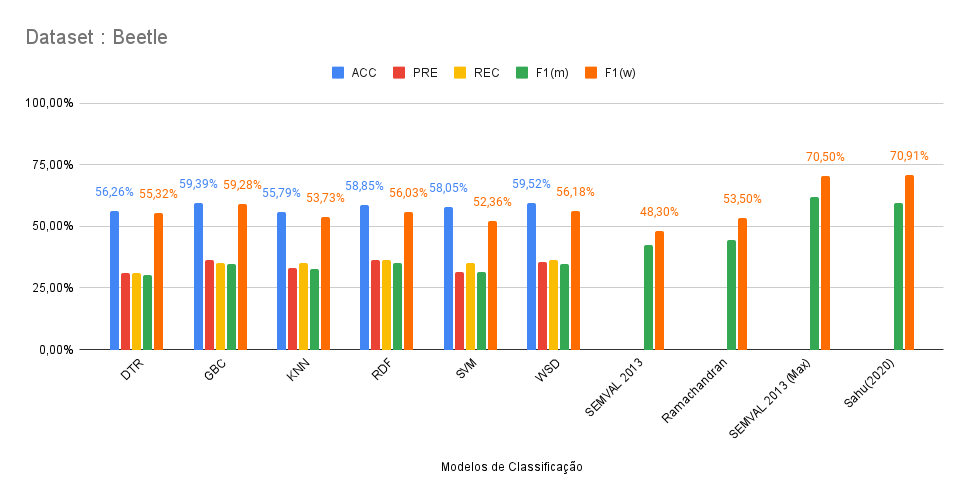
\includegraphics[width=\textwidth]{figuras/Beetle-75.png}

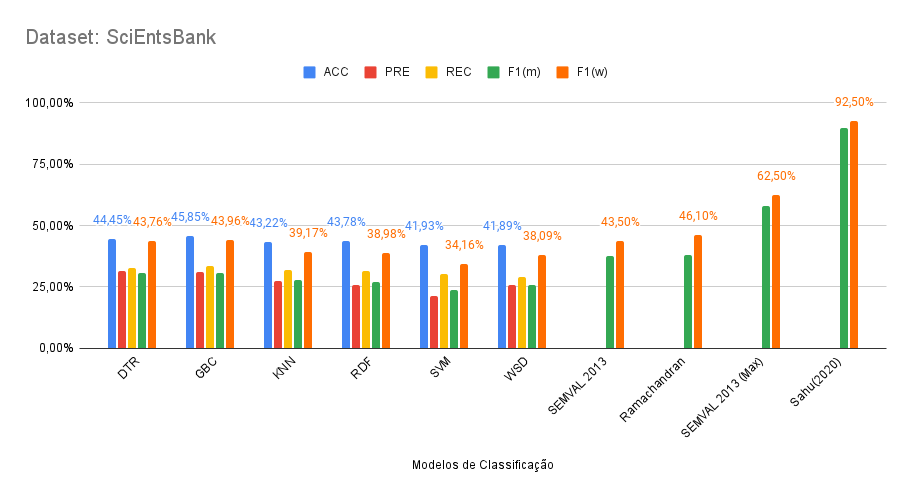
\includegraphics[width=\textwidth]{figuras/SciEntsBank-75.png}
\caption{Resultados obtidos nos \textit{datasets Beetle} e \textit{SciEntsBank} pelos classificadores em comparação com os principais encontrados na literatura.}
\label{fig-semeval75}
\end{figure}

Na Figura \ref{fig-semeval75}, os gráficos destacam os valores obtidos nas métricas F1-macro e F1-ponderado conforme os principais resultados da literatura \cite{dzikovska2013, ramachandran2015a,sahu2020}. Conforme os trabalhos da literatura, evidenciamos a distância dos resultados obtidos em relação ao que foi apresentado como o \textit{estado da arte} neste cenário. Apesar disso, ambos os resultados são superiores ao \textit{baseline} proposto. Nesta perspectiva, abordagens com a criação de modelos de resposta, utilizando informações adicionais sobre o tema ou expressões regulares, sobressaem com melhor desempenho mas, em geral, demandam maior esforço do professor \cite{ramachandran2015a, sahu2020}. No entanto, isto indica que tais estratégias seguem um único viés de resposta, tornando-se menos efetivas ao lidar com variações linguísticas \cite{filighera2020}.

Ainda, temos dentre as 4380 respostas do \textit{Beetle} 1841 anotadas como \textit{correct}, 1160 como \textit{contradictory} e 1031 como \textit{partially-correct-incomplete}. Por outro lado, apenas 218 foram avaliadas como \textit{non-domain} e 130 como \textit{irrelevant}. Considerando ainda a distribuição de classes, a situação é agravada em relação ao \textit{SciEntsBank}. Dentre as 5509 respostas, 2241 foram dadas como \textit{correct}, 1437 como \textit{partially-correct-incomplete}, 1248 como \textit{irrelevant} e 557 como \textit{contradictory}. Só constam neste \textit{dataset} 26 respostas anotadas como \textit{non-domain} dentre as 143 questões. Notoriamente, são poucas amostras para algumas categorias que se destacam quando vemos que, em média, o primeiro \textit{dataset} apresenta 93 respostas por questão enquanto o segundo apresenta apenas 38 respostas. Portando, apesar da complexidade de avaliar tal questão, os resultados são positivos, aprimorando resultados esperados conforme a distribuição de \textit{clusters}.

Em outra perspectiva, com dados discretos, analisamos os resultados dos \textit{datasets Open University}, \textit{Powergrading} e \textit{Kaggle ASAP-SAS}. Inicialmente abordaremos o \textit{dataset} da \textit{Open University}, por conta do formato de anotação. Neste conjunto de dados a cada resposta foi designada a nota 0 ou nota 1, como respostas corretas ou incorretas. Bem distinta dos \textit{datasets Beetle} e \textit{SciEntsBank}, este conjunto contém mais de 23 mil respostas e, em média, 1190 respostas para cada questão. Isso impacta diretamente na construção de modelos de resposta, com uma variedade de padrões para uma mesma classe, sendo possível a identificação de núcleos de resposta bem consistentes segundo a simetria da classe. Os resultados apresentados na Tabela \ref{tab-OU75} refletem justamente este aspecto.

\begin{table}[!h]
\begin{center}
\begin{tabular}{l r r r r r r r}
    \hline
    \multicolumn{7}{l}{\textbf{Open University}} &  (2 Categorias) \\ \hline
     & \multicolumn{7}{c}{M{\'e}tricas} \\ \cline{2-8}

     & ACC & PRE & REC & F1(m) & F1(w) & Kappa(ln) & Kappa(qu) \\ \cline{2-8}
DTR & 95,39\% & 90,37\% & \textbf{91,96\%} & 90,83\% & 94,86\% & 0,8053 & 0,8053 \\
GBC & \textbf{96,15\%} & \textbf{93,69\%} & 91,68\% & \textbf{92,01\%} & \textbf{95,51\%} & \textbf{0,8317} & \textbf{0,8317} \\
KNN & 89,41\% & 84,82\% & 82,60\% & 82,60\% & 88,52\% & 0,6264 & 0,6264 \\
RDF & 92,69\% & 89,41\% & 89,04\% & 86,86\% & 92,92\% & 0,7344 & 0,7344 \\
SVM & 86,46\% & 79,15\% & 77,07\% & 74,81\% & 82,98\% & 0,5093 & 0,5093 \\
WSD & 80,62\% & 74,53\% & 71,29\% & 70,16\% & 78,43\% & 0,3788 & 0,3788 \\

    \hline
    \hline
\end{tabular}
\end{center}
\caption{Resultados de classificação para o \textit{dataset OpenUniversity}.}
\label{tab-OU75}
\end{table}

É evidente, através dos resultados em destaque na Tabela \ref{tab-OU75}, que a grande quantidade de padrões de nota aumentam consideravelmente a qualidade de classificação. Com ACC de 96,15\%, o algoritmo GBC captura detalhes nas respostas e formas de avaliação muito próximas do modelo do professor. Por conta disso, podemos dizer que a captura das estruturas de linguagem analisadas foram de alta qualidade. Com isso, o sistema um classificador retorna um excelente modelo de avaliação, compatível com as expectativas do professor. De acordo com as classes, os classificadores GBC, RDF e DT apresentam F1-ponderado acima de 90\%. A Figura \ref{fig-OU75} apresenta os resultados obtidos neste \textit{dataset} em relação aos descritos pelos autores em sua publicação \cite{butcher2010}.

\begin{figure}[!h]
\centering
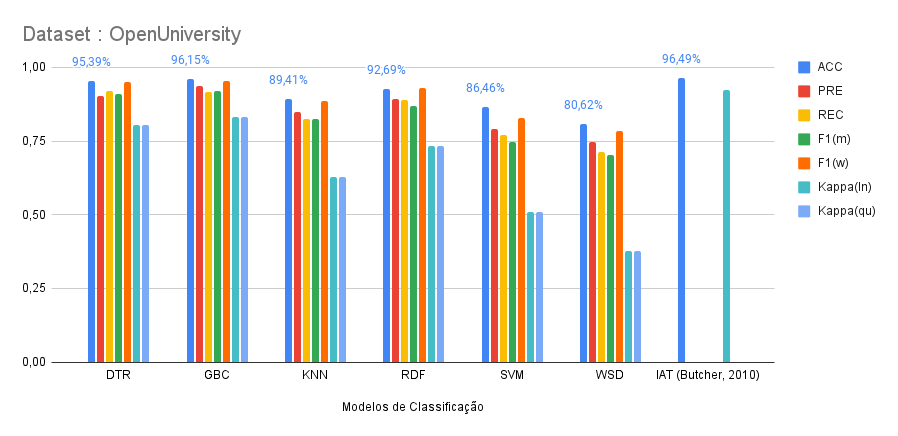
\includegraphics[width=\textwidth]{figuras/OU-75.png}
\caption{Comparação do sistema dos autores do \textit{dataset Open University} em relação ao \textit{p}Nota.}
\label{fig-OU75}
\end{figure}

A Figura \ref{fig-OU75} caracteriza a proximidade do modelo GBC do \textit{p}Nota com o \textit{IAT}, sistema aplicado na \textit{Open University}. Como o artigo destaca, o sistema tem conhecimento sobre o conteúdo e regras de associação de respostas com o tema para a produção de \textit{feedbacks} direcionados. Portanto, tal trabalho contém uma base de conhecimento sobre o tema para além do que é formado pelas atividades. Entretanto, apenas com os exemplos anotados, o \textit{p}Nota produz um modelo consistente, com desempenho equivalente aos modelos voltados ao tema.

Anotado de forma similar ao \textit{Open University}, o \textit{dataset Powergrading} também contém respostas avaliadas de forma binária (correto 1 ou incorreto 0). Porém, o \textit{Powergrading} é avaliado por três avaliadores. Com as notas binárias, o objetivo é atender o resultado coincidente entre os avaliadores humanos. O desempenho obtido pelo \textit{p}Nota neste \textit{dataset} é caracterizado na Tabela \ref{tab-PG75}.

\begin{table}[!h]
\begin{center}
\begin{tabular}{l r r r r r r r}
    \hline
    \multicolumn{7}{l}{\textbf{Powergrading}} &  (2 Categorias) \\ \hline
     & \multicolumn{7}{c}{M{\'e}tricas} \\ \cline{2-8}

     & ACC & PRE & REC & F1(m) & F1(w) & Kappa(ln) & Kappa(qu) \\ \cline{2-8}
DTR & 99,37\% & 92,62\% & 91,91\% & 92,19\% & 99,27\% & 0,8444 & 0,8444 \\
GBC & \textbf{99,49\%} & 93,77\% & \textbf{91,97\%} & \textbf{92,53\%} & \textbf{99,37\%} & \textbf{0,8515} & \textbf{0,8515} \\
KNN & 99,31\% & 89,66\% & 90,00\% & 89,82\% & 98,98\% & 0,8000 & 0,8000 \\
RDF & 99,37\% & \textbf{94,68\%} & 90,50\% & 90,75\% & 99,11\% & 0,8173 & 0,8173 \\
SVM & 99,37\% & \textbf{94,68\%} & 90,50\% & 90,75\% & 99,11\% & 0,8173 & 0,8173 \\
WSD & 99,03\% & 90,39\% & 90,32\% & 90,33\% & 98,90\% & 0,8074 & 0,8074 \\

    \hline
    \hline
\end{tabular}
\end{center}
\caption{Resultados de classificação para o \textit{dataset Powergrading}.}
\label{tab-PG75}
\end{table}

A Tabela \ref{tab-PG75} aponta o desemepenho dos classificadores no \textit{dataset Powergrading}, inclusive superiores a média de 90\% em CA (voto majoritário). Nesse aspecto, todos os 6 classificadores apresentam ACC e F1-ponderado acima de 99\%, reflexo direto da homogeneidade dos \textit{clusters}formados na etapa anterior \cite{basu2013}. Em aspecto similar ao observado no \textit{dataset Open University}, com muitas amostras os modelos das classes se tornam muito consistentes. Os resultados observados ficam evidentes na Figura \ref{fig-PG75}.

\begin{figure}[!h]
\centering
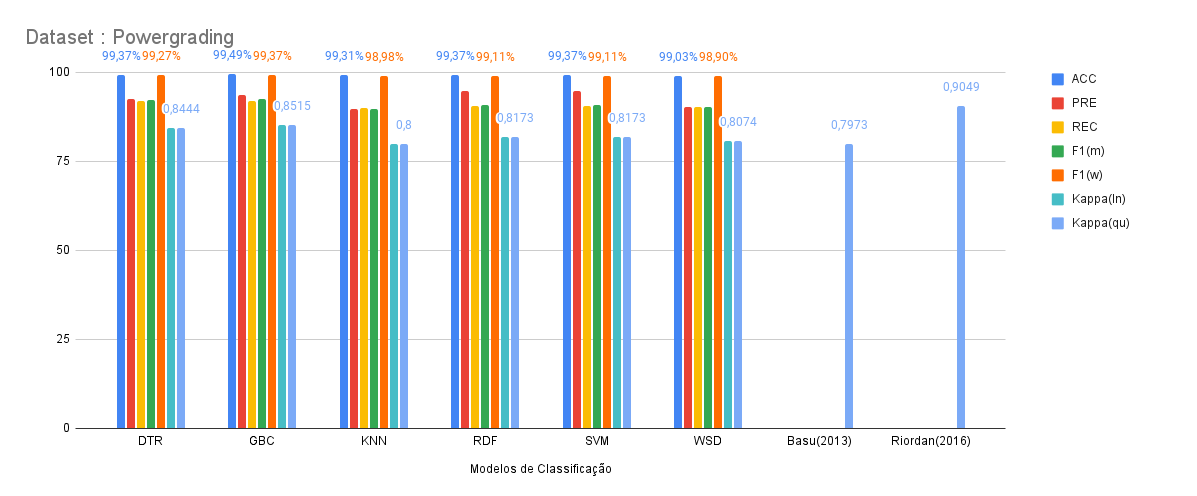
\includegraphics[width=\textwidth]{figuras/Powergrading-75}
\caption{Resultados dos classificadores com dados do \textit{dataset Powergrading}.}
\label{fig-PG75}
\end{figure}

Podemos, através da Figura \ref{fig-PG75}, destacar a relação da \textit{clusterização} na amostragem para o classificador. Apresentando textos restritos ao tema, sucintos e em \textit{clusters} homogêneos, são formados classificadores com alto desempenho. Deste modo, com modelos bem definidos nas etapas de \textit{clusterização} e classificação produzimos avaliadores SAG muito similares ao tutor. Por outro lado, em alguns \textit{datasets} a diversidade textual, a característica das notas atribuídas, os modelos linguísticos e a expectativa de resposta influenciam muito na capacidade do avaliador automático. Todas estas características são evidenciadas com conteúdos mais complexos, como a base de dados da competição do \textit{Kaggle ASAP-SAS}.



\begin{comment}

Edição a partir daqui
\end{comment}


Em outra perspectiva, temos o \textit{dataset} da \textit{University of North Texas} da avaliação com poucos dados. Neste conjunto, cada questão contém 30 respostas. Todas as perguntas são referentes a disciplina de Estrutura de Dados do curso de Ciência da Computação. Assim, como os demais procedimentos, sem usar respostas candidatas, utilizamos a amostragem através dos grupos resultantes da \textit{clusterização}. Foi avaliada a atribuição de notas para três anotações do conjunto de dados: \textit{Avaliador1}, \textit{Avaliador2} e a \textit{Média}. Os resultados obtidos com os algoritmos de regressão LINR, LSSR, KNRG, DTRG, WSRG na atribuição de notas entre 0 e 5 são apresentados na Tabela \ref{tab-UNT75}.

\begin{table}[!h]
\begin{center}
\begin{tabular}{p{5cm} r r r }
    \hline
    \multicolumn{4}{l}{\textbf{University of North Texas} (Notas 0 - 5)} \\ \hline
     & \multicolumn{3}{c}{M{\'e}tricas} \\

    & \multicolumn{3}{l}{Avaliador1} \\ \cline{2-4}
 & MAE & MSE & RMSE \\
LINR & 1,0066 & \textbf{2,5069} & \textbf{1,1955} \\
LSSR & 1,3273 & 3,1713 & 1,4712 \\
KNRG & 0,9366 & 2,9032 & 1,2557 \\
DTRG & \textbf{0,9233} & 3,7338 & 1,4482 \\
WSRG & 1,2832 & 3,0113 & 1,4240 \\
\\
& \multicolumn{3}{l}{Avaliador2} \\ \cline{2-4}
 & MAE & MSE & RMSE \\
LINR & \textbf{0,4752} & \textbf{0,6099} & \textbf{0,6119} \\
LSSR & 0,6502 & 0,8605 & 0,7640 \\
KNRG & 0,4917 & 0,7550 & 0,6658 \\
DTRG & 0,5121 & 1,2002 & 0,7856 \\
WSRG & 0,6523 & 0,8839 & 0,7680 \\
\\
& \multicolumn{3}{l}{Média} \\ \cline{2-4}
 & MAE & MSE & RMSE \\
LINR & \textbf{0,5058} & \textbf{0,5476} & \textbf{0,6199} \\
LSSR & 0,7299 & 0,8464 & 0,8170 \\
KNRG & 0,5055 & 0,6804 & 0,6765 \\
DTRG & 0,5811 & 1,1244 & 0,8372 \\
WSRG & 0,7024 & 0,8088 & 0,7920 \\

    \hline
    \hline
\end{tabular}
\end{center}
\caption{Índices de erro para cada algoritmos de regressão resultantes de cada um dos três cenários de avaliação do \textit{dataset} da \textit{University of North Texas}.}
\label{tab-UNT75}
\end{table}

A Tabela \ref{tab-UNT75} detalha o desempenho de cada algoritmo de regressão para as métricas MAE, MSE e RMSE. Nos resultados, destacamos a divergência entre avaliadores, com o \textit{Avaliador 1} sendo mais irregular na análise do sistema. Por outro lado, observando os classificadores, ressaltamos a capacidade de reconhecimento de padrões mais efetiva aos modelos do \textit{Avaliador 2} e da \textit{Média}. A diferença entre os melhores resultados se destacam, para o primeiro avaliador obtemos RMSE de 1,1930 pontos. Enquanto isso, para o segundo obtemos RMSE de 0,6099 pontos, uma queda de 0,5831 pontos. Neste conjunto de dados, conforme a literatura, o RMSE foi utilizado como padrão para comparações com os demais trabalhos, buscando minimizar o erro obtido de acordo com a nota média. As Figuras \ref{fig-UNT-Err} e \ref{fig-UNT-RMSE} detalham os erros encontrados para as três métricas por cada um dos algoritmos e a comparação com o RMSE dos trabalhos da literatura.

\begin{figure}[!h]
\begin{minipage}[t]{.5\textwidth}
 \centering
 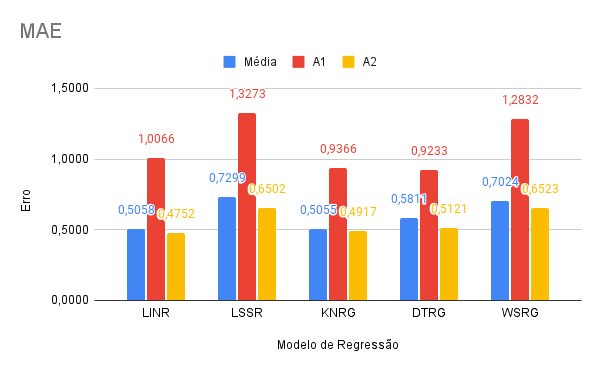
\includegraphics[width=\textwidth]{figuras/UNT-MAE.png}
\end{minipage}
\hfill
\begin{minipage}[t]{.5\textwidth}
 \centering
 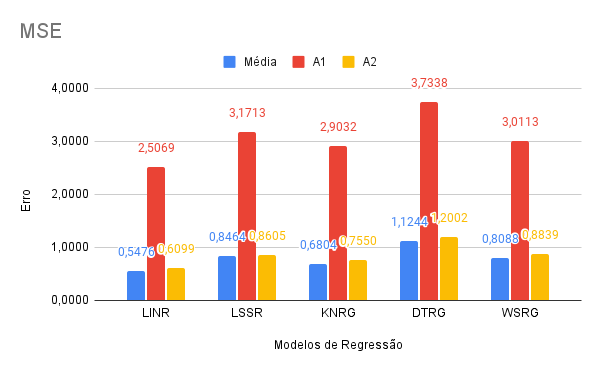
\includegraphics[width=\textwidth]{figuras/UNT-MSE.png}
\end{minipage}
\caption{Índices de MAE e MSE para os algoritmos testados em cada um dos três cenários de avaliação do \textit{dataset} da \textit{University of North Texas}.}
\label{fig-UNT-Err}
\end{figure}

\begin{figure}[!h]
\centering
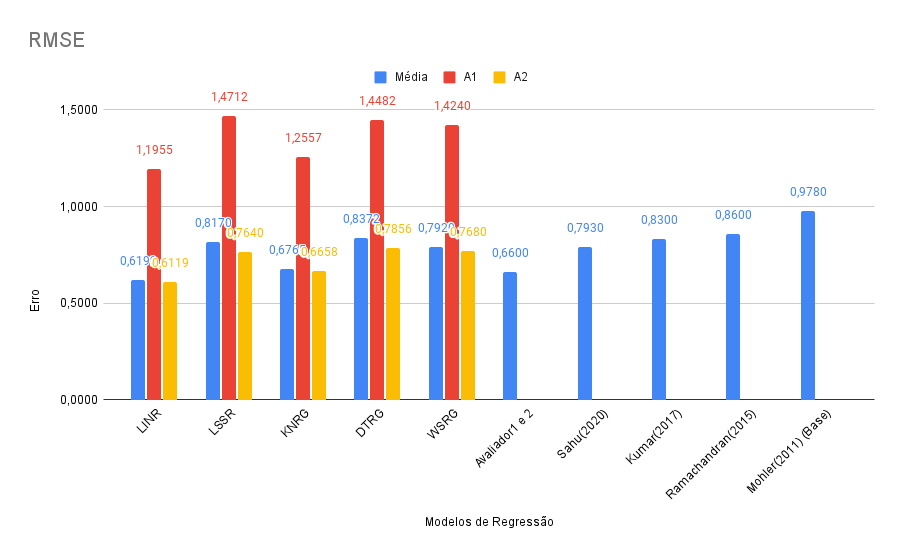
\includegraphics[width=\textwidth]{figuras/UNT-RMSE}
\caption{Comparação entre o índice de RMSE obtidos pelo sistema e modelos propostos na literatura.}
\label{fig-UNT-RMSE}
\end{figure}

Como as Figuras \ref{fig-UNT-Err} e \ref{fig-UNT-RMSE} ilustram, existe uma grande diferença entre os avaliadores. O erro observado entre humanos em RMSE é de 0,66 pontos \cite{mohler2011}. Em uma comparação com demais métodos de avaliação, podemos destacar os excelentes resultados obtidos com o algoritmo de regressão linear simples LINR, como o melhor em todos os três cenários. Entretanto, dentre os algoritmos de regressão testados observamos consistência entre resultados, com pequenas variações entre os algoritmos. Enquanto na literatura o menor resultado observado é de 0,793 em RMSE, alcançamos resultados de 0,617 com LINR, seguido pelo KNRG com 0,677 pontos. Dada a avaliação com base no alinhamento com a resposta candidata elaborada pelo professor, os resultados obtidos reforçam que o uso da amostragem na produção do critério avaliativo pode ser muito efetivo. Assim, o estudo da distribuição de amostras torna o sistema conhecedor da dinâmica de avaliação realizando, neste caso, a interpolação em um espectro de notas conhecido. Esse nível, apesar da amostragem pré-estabelecida, caracteriza-se por um RMSE bem abaixo do observado até o momento na literatura \cite{ramachandran2015b, kumar2017, sahu2020}.





Adicionalmente, utilizamos dados \textit{Projeto Feira Literária} para ilustrar os resultados em dados nacionais. Em português, tais dados são um comparativo direto aos resultados obtidos em dados do exterior. Este dado foi coletado em conjunto com os autores para descrição da aplicação do \textit{p}Nota e seu uso por professores \cite{nascimento2020}. Este caracteriza-se pela presença de erros de escrita e conteúdos fora de tópico, sendo fatores avaliados negativamente pelo tutor. A Tabela \ref{tab-findes75} caracteriza o desempenho de cada um dos seis classificadores e seus resultados alcançados na avaliação das questões do projeto.

\begin{table}[!h]
\begin{center}
\begin{tabular}{l r r r r r r r}
    \hline
    \multicolumn{7}{l}{\textbf{Projeto Feira Liter{\'a}ria}} & (4 Categorias) \\ \hline
     & \multicolumn{7}{c}{M{\'e}tricas} \\ \cline{2-8}

    \input{tabelas/tab-findes75.tex}

    \hline
    \hline
\end{tabular}
\end{center}
\caption{Resultados de classificação para o \textit{Projeto Feira Literária}.}
\label{tab-findes75}
\end{table}

Conforme a Tabela \ref{tab-findes75}, observamos que dos seis classificadores testados, três apresentam resultados de boa qualidade. Apesar dos desafios do conjunto de dados, os algoritmos RDF, WSD e GBC apresentam resultados superiores a 60\% em ACC e F1-ponderado. Com 70 respostas e a pluralidade de estruturas textuais encontradas, destacamos a similaridade entre o desafio de correção dos datasets \textit{Beetle} e \textit{SciEntsBank} no ensino de ciências. Porém, podemos ressaltar como uma diferença melhores índices de PRE, REC e F1-macro. Podemos observar através da Figura \ref{fig-findes75} a proximidade destes índices com o grau de ACC alcançado.

\begin{figure}[!h]
\centering
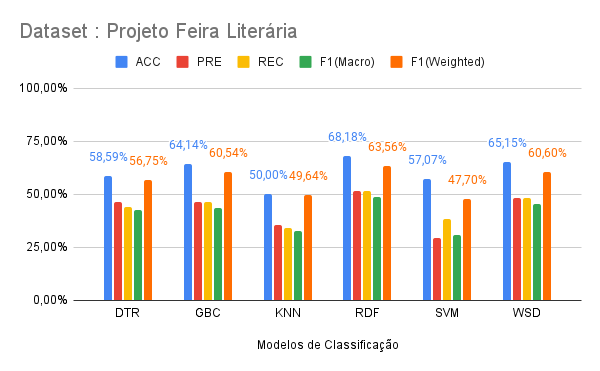
\includegraphics[width=\textwidth]{figuras/Findes-75}
\caption{Resultados alcançados para os classificadores com dados em português do \textit{Projeto Feira Literária}.}
\label{fig-findes75}
\end{figure}

Nessa perspectiva, a Figura \ref{fig-findes75} representa um equilíbrio dos classificadores na produção de modelos por nota e a avaliação em geral de cada categoria. Quatro classificadores, RDF, WSD, GBC e DTR, apresentam alto desempenho, enquanto KNN e SVM destoam com resultados inferiores a 50\% em F1-ponderado. Portanto, os modelos avaliativos gerados demonstram complexidade mas em geral têm bons resultados.


\subsection{Resultados de \textit{Amostragem}}
\label{sec-res-amostragem}


\section{Discussão de Resultados}
\label{sec-discussao}

Os sistemas SAG têm características interessantes e de grande complexidade. Ao tempo que é um desafio lidar com diferentes tamanhos e padrões de resposta, ainda existem grande impacto o critério de avaliação. O desbalanceamento entre classes, os múltiplos padrões de resposta e a baixa quantidade de exemplos tornam complexa a criação de modelos avaliativos robustos.

De qualquer forma, por conta da dinâmica de avaliação própria de cada questão, vemos dentro de cada base de dados múltiplas perspectivas. Enquanto parte destoa com dificuldade no processo avaliativo, outras questões apresentam alto desempenho avaliativo com qualidade superior até a avaliação entre humanos. Um destaque no método avaliativo do \textit{p}Nota quando comparado à demais abordagens da literatura é a capacidade de processamento em várias linguagens. Nesse aspecto, a adaptabilidade do sistema com a análise personalizada da estrutura linguística caracteriza-se como um diferencial das abordagens mais recentes. Em sua aplicação, o sistema demanda entre 5 minutos e 6 horas de processamento conforme o número de características e amostras do conjunto de dados, desconsiderando o processo de anotação do professor. Logo, é fundamental adequar o sistema ao uso cotidiano do tutor e seu ritmo de correção, tendo em vista a entrega rápida de resultados em sala.

Na criação do modelo linguístico, os sistemas trabalham o alinhamento entre o conjunto de respostas e as respostas candidatas. Entretanto, a proposta apresentada neste trabalho busca a evolução do modelo criado iterativamente com a avaliação do professor. Para além da análise textual o sistema prioriza a conexão entre conteúdo e critério avaliativo. Deste modo, as nuances textuais interpretadas pelo tutor durante a avaliação são destacadas com o modelo estabelecido no modelo de atribuição de notas. Superdimensionados para a avaliação de uma determinada disciplina ou tema, os modelos rígidos divergem bastante da aplicação dos sistemas SAG no cotidiano do professor. Assim, o tutor espera que o sistema seja capaz de reduzir o esforço de correção, dando suporte ao seu método assim que requisitado. Portanto, independente do cenário ao qual é aplicado, o sistema SAG deve lidar com as respostas buscando minorar a demanda de verificação do conteúdo caracterizando as demandas de ensino-aprendizagem.

Além disso, ainda é importante salientar que, apesar de serem comuns os modelos rígidos, direcionados a domínios específicos ou dependentes de regras, o modelo proposto neste trabalho foi o mesmo aplicado para todas as questões. Por conta disso, inclui-se na qualidade dos resultados obtidos a capacidade do próprio sistema na adaptação ao tema e ao modelo de avaliação. Nesta linha, poucos parâmetros são passados, tornando o sistema uma cadeia de decisões sobre o processo. A lista completa de parâmetros está no Capítulo \ref{manual-pNota}.

Portanto, a escolha dos modelos segundo seu alinhamento com a avaliação humana acrescenta fluidez no processo de correção. Tornamos o modelo flexível para que, cada modelo seja utilizado nas situações ao qual melhor se adequa. O nível de adequação entre o modelo e a expectativa do professor é dada através das medidas de correlação de \textit{Pearson} ou coeficiente \textit{Kappa}. A tendência, então, é que os métodos de classificação ou de regressão selecionados sejam os que tem desempenho superior, com o professor auditando os resultados realizando apenas pequenos ajustes.